%!TEX TS-program = pdflatex                                          %
%!TEX encoding = UTF8                                                %
%!TEX spellcheck = en-US                                             %
%
%%%%%%%%%%%%%%%%%%%%%%%%%%%%%%%%%%%%%%%%%%%%%%%%%%%%%%%%%%%%%%%%%%%%%%
% Handout_ModelingStructuralLesions.tex
% A handout to follow during the hands-on sessions 
% 
% Authors: Timothée Proix
% 
% 
%%%%%%%%%%%%%%%%%%%%%%%%%%%%%%%%%%%%%%%%%%%%%%%%%%%%%%%%%%%%%%%%%%%%%%
% based on the tufte-latex template                                  %

\documentclass{tufte-handout}

%\geometry{showframe}% for debugging purposes -- displays the margins

\usepackage{amsmath}

% Set up the images/graphics \underline{\textbf{Analysis}}
\usepackage[pdftex]{graphicx}
\setkeys{Gin}{width=\linewidth,totalheight=\textheight,keepaspectratio}
\graphicspath{{figures/} {../../framework_tvb/tvb/interfaces/web/static/style/img/} {../../framework_tvb/tvb/interfaces/web/static/style/img/nav/}}

\title{The Virtual Brain: Hands on Session \#3}
\date{7th June 2014} 

% The following package makes prettier tables.  
\usepackage{booktabs}


% The units package provides nice, non-stacked fractions and better spacing
% for units.
\usepackage{units}
\usepackage[svgnames]{xcolor}

% The fancyvrb package lets us customize the formatting of verbatim
% environments.  We use a slightly smaller font.
\usepackage{fancyvrb}
\fvset{fontsize=\normalsize}

% Small sections of multiple columns
\usepackage{multicol}

% For adjustwidth environment
\usepackage[strict]{changepage}

% For formal definitions
\usepackage{framed}

% And some maths
\usepackage{amsmath}  % extended mathematics

% Resume a list
\usepackage{enumitem}

% Background image

\usepackage{wallpaper}

% Provides paragraphs of dummy text
\usepackage{lipsum}

% These commands are used to pretty-print LaTeX commands
\newcommand{\doccmd}[1]{\texttt{\textbackslash#1}}% command name -- adds backslash automatically
\newcommand{\docopt}[1]{\ensuremath{\langle}\textrm{\textit{#1}}\ensuremath{\rangle}}% optional command argument
\newcommand{\docarg}[1]{\textrm{\textit{#1}}}% (required) command argument
\newenvironment{docspec}{\begin{quote}\noindent}{\end{quote}}% command specification environment
\newcommand{\docenv}[1]{\textsf{#1}}% environment name
\newcommand{\docpkg}[1]{\texttt{#1}}% package name
\newcommand{\doccls}[1]{\texttt{#1}}% document class name
\newcommand{\docclsopt}[1]{\texttt{#1}}% document class option name

\newcommand\blfootnote[1]{\begingroup
         \renewcommand\thefootnote{}\footnote{\phantom{\thefootnote} #1}%
         \addtocounter{footnote}{-1}%
         \endgroup
          }

% Colours: environment derived from framed.sty: see leftbar environment definition
\definecolor{formalshade}{rgb}{0.95,0.95,1}
\definecolor{simulationshade}{rgb}{0.92, 1.0, 0.95}

% Title rule
\newcommand{\HRule}{\rule{\linewidth}{0.5mm}}

% Framed  coloured boxes

%% Blue box: for steps regarding analysis and such
\newenvironment{formal}{%
  \def\FrameCommand{%
    \hspace{1pt}%
    {\color{DarkBlue}\vrule width 2pt}%
    {\color{formalshade}\vrule width 4pt}%
    \colorbox{formalshade}%
  }%
  \MakeFramed{\advance\hsize-\width\FrameRestore}%
  \noindent\hspace{-4.55pt}% disable indenting first paragraph
  \begin{adjustwidth}{}{7pt}%
  \vspace{2pt}\vspace{2pt}%
}
{%
  \vspace{2pt}\end{adjustwidth}\endMakeFramed%
}

%% Green box: for steps regarding simulatio **only**
\newenvironment{simulation}{%
  \def\FrameCommand{%
    \hspace{1pt}%
    {\color{ForestGreen}\vrule width 2pt}%
    {\color{simulationshade}\vrule width 4pt}%
    \colorbox{simulationshade}%
  }%
  \MakeFramed{\advance\hsize-\width\FrameRestore}%
  \noindent\hspace{-4.55pt}% disable indenting first paragraph
  \begin{adjustwidth}{}{7pt}%
  \vspace{2pt}\vspace{2pt}%
}
{%
  \vspace{2pt}\end{adjustwidth}\endMakeFramed%
}

%% Orange box: for verbose descriptions
\newenvironment{blah}{%
  \def\FrameCommand{%
    \hspace{1pt}%
    {\color{DarkOrange}\vrule width 2pt}%
    {\color{PeachPuff}\vrule width 4pt}%
    \colorbox{PeachPuff}%
  }%
  \MakeFramed{\advance\hsize-\width\FrameRestore}%
  \noindent\hspace{-4.55pt}% disable indenting first paragraph
  \begin{adjustwidth}{}{7pt}%
  \vspace{2pt}\vspace{2pt}%
}
{%
  \vspace{2pt}\end{adjustwidth}\endMakeFramed%
}

%%%%%%%%%%%%%%%%%%%%%%%%%%%%%%%%%%%%%%%%%%%%%%%%%%%%%%%%%%%%%%%%%%%%%%%%%%%%%%
%                      The document starts here                              %
%%%%%%%%%%%%%%%%%%%%%%%%%%%%%%%%%%%%%%%%%%%%%%%%%%%%%%%%%%%%%%%%%%%%%%%%%%%%%%
\begin{document}
\thispagestyle{plain}
\LLCornerWallPaper{1.5}{background.png}
\begin{titlepage}
\begin{center}
% Upper part of the page. The '~' is needed because \\
% only works if a paragraph has started.

\includegraphics[width=1.5\textwidth]{./tvb_logo_transparent_square.png}~\\[0.5cm]

% Title
\begin{fullwidth}
\HRule \\[0.2cm]
\begin{center}
{ \huge \bfseries Hands-on Session \#1 \\ [0.2cm] Building Your Own Brain Network Model \\[0.1cm] }
{ \large \bfseries June 7, 2014 \\[0.2cm]}
\end{center}
\HRule \\[0.2cm]
\end{fullwidth}

\end{center}
\end{titlepage}
\newpage
\ClearWallPaper


\begin{abstract}
\noindent A small paragraph that gives context to the session, that is, 
why we are modeling this particular case.\\
The aim is to model specific patients whos data we get from neuroimaging methods and to reproduce one or several modalities . then we can try 
1) to ifind epileptogenic regions (concorance with data) 
2) to model chirugy cases and impact on the conectomr
\end{abstract}

%\printclassoptions

%\begin{fullwidth} % uncomment this environment to get full texwidth paragraphs 
 
%\end{fullwidth}

\section{Objectives}\label{sec:objectives}
from clinical point of view, see summary
The main goal of this session is to provide a clear understanding of how wen can put apatient i tvb, model the different modalities and perform soe anaylis on the results and/or export the results

Furthemore, we probably need to provide one or two references about relevant
empirical studies ...


\subsection{What's inside Project X }\label{sec:project_data}

The table should list the data inside a project. 
We provide data for simulation taken from the Human Connectom Project. Data were handled with the pipeline described earlier today.

\begin{margintable}
  \centering
  \fontfamily{ppl}\selectfont
  \begin{tabular}{ll}
    \toprule
    Datatype & Sumary info                       \\
    \midrule
    Connectivity         & \unit[X]{nodes}                    \\
    Surface              & \unit[15000 x 3]{vertices}     \\
    RegionMapping        & \unit[15000]{nodes}            \\
    EEGProjectionMatrix     & \unit[M x N]{sources x sensors} \\
    EEGSensors              & \unit[N x 4]{sensors x coordinates} \\
    MEGProjectionMatrix     & \unit[M x N]{sources x sensors} \\
    MEGSensors              & \unit[N x 4]{sensors x coordinates}\\
    IntracranialSensors     & \unit[N x 4]{sensors x coordinates} \\
    TimesSeries          & \unit[5000]{ms} \\
    \bottomrule
  \end{tabular}
  \caption{Here are the datatypes included in Project X}
  \label{tab:margintab}
\end{margintable}

In this table you will find the different simluations in the project.
\begin{margintable}
  \centering
  \fontfamily{ppl}\selectfont
  \begin{tabular}{l}
    \toprule
    Name \\
    \midrule
    \textit{EvokedResponses\_init} \\
    \textit{EvokedResponses\_init\_branch1}  \\ 
    \textit{EvokedResponses\_init\_stochastic}  \\ 
    \textit{EvokedResponses\_init\_stochastic}  \\ 
    \textit{EvokedResponsesSurface\_init} \\
    \textit{EvokedResponsesSurface\_init\_branch1} \\
     \textit{EvokedResponsesSurface\_init\_branch2} \\
     \textit{HomogeneousRegionModel}\\
     \textit{HeterogeneousRegionModel} \\
     \textit{HomogeneoussSurfaceModel}\\
     \textit{HeterogeneousSurfaceModel}\\
    \bottomrule
  \end{tabular}
  \caption{Simulations in this project.}
  \label{tab:normaltab}
\end{margintable}

% let's start a new thought -- a new section

\newthought{In this session}, we'll only go through the necessary steps
required to reproduce the data described in Table~\ref{tab:margintab}.
Describe some particularities of the project. 


\subsection{Steps: importing the data}\label{sec:import}

In your browser go to the tab that says \textsc{project}.
Figure~\ref{fig:fig} shows a snapshots of this working area.
At first step, we will import all the relevant modaliites.

A little word on the pipeline here.

Show how to import data

As a first step, you we will explore {\color{RoyalBlue}\textsc{A}}. Then, we
will do {\color{RoyalBlue} \textsc{B}} to achieve
{\color{RoyalBlue} \textsc{C}}.





\subsection{Steps: exploring the epileptor model}\label{sec:epileptor}

Before doing any simulations, we would like to have a look at the phase space of the Epileptor model
to understand better his dynamics, as you have seen in Session IV.

\begin{formal}
  \begin{enumerate}[resume]
  \item Go to simulator and select the Epileptor model
  \item Click on Set Up Region Model.
  \item Look at the phase space (Fig. \ref{fig:phase_space}). We have here the first population (variables y0 and y1).
  The left most intersection of the nullcline defines a stable fix point whereas the rightmost intersection 
  is the center of a limit cycle. Both states are separated by a separatrix, as you can say by trying different trajectories
  in this phase space (left click on the figure) limit cycle.
  \item Now change the value of the parameter $x_0$ to the value -2.2 and see what happens to the phase space: the cubic nullcline
  is raised such that only the leftmost fix piont now exist. The model becomes non-epileptogenic.
  \item You can also look at the phase space for other variables, such as y2 against y0 (slow-fast subsystem) or y5 against y4 (second population)
  \end{enumerate}
\end{formal}


\begin{figure}[h]
  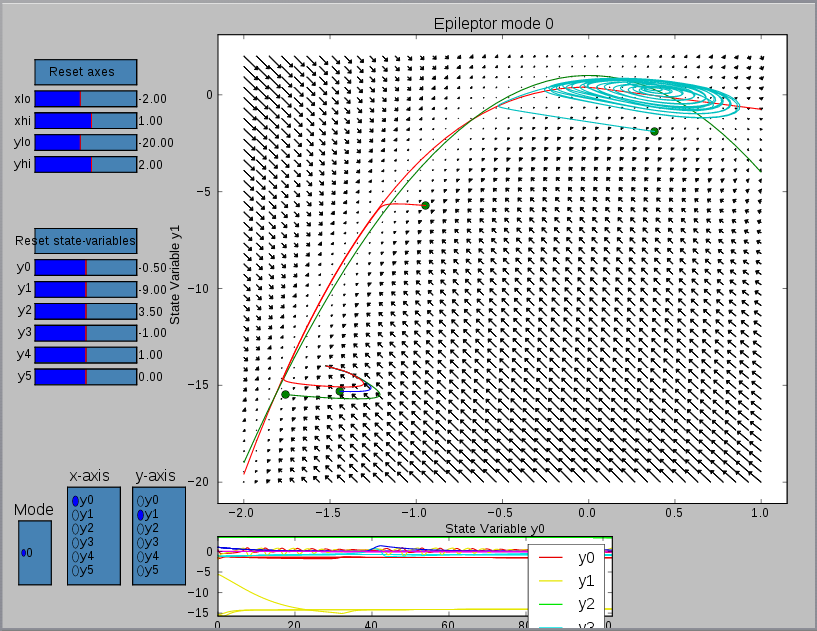
\includegraphics[width=\linewidth]{Handout_UI_ModellingAnEpilepticPatient_PhaseSpace}%
  \caption{phase space for the first population}%
  \label{fig:phase_space}%
\end{figure}
\subsection{Steps: Preparing a region parameter exploration }

We are going to model a patient with temporal lobe epilepsy. For this we are going to choose epileptogenic region, i.e. 
introduce heterogeneity in the Epileptor parameters such as seen in Session IV. We choose epileptic regions in the right limbic areas 
(right hippocampus (rHC), parahippocampus (rPHC) and amygdala (rAMYG). We also add two regions as epileptogenic, but closer
to the threshold : the superior temporal cortex (rTS) and the ventral temporal cortex (rTV)

\begin{simulation}
  \begin{enumerate}
  \item Still in the same page: all nodes are selected by default, give them the value -2.2 for the $x_0$ parameter.
  \item Now remove all, select lHC, lAMYG and lPHC, save the selection 
	and set the parameter $x_0$ to the value -1.6. Submit the parameter values.
  \item Configure the view and add a brain viewer and a fourier spectrum, then save your choices.
  \item Choose an integration step size of 0.1, a raw monitor and 6000 as a simulation length. All the other parameters area
  given in the table \ref{tab:modeltab}.
 \end{enumerate}
\end{simulation}

\begin{margintable}
  \centering
  \fontfamily{ppl}\selectfont
  \begin{tabular}{ll}
    \toprule
    Model parameter & Value \\
    \midrule
             $Iext$          &   3.1  \\
             $Iext2$          &  0.45   \\
             $R$           &   0.00035        \\
             $slope$           &   0.0   \\
    \bottomrule
  \end{tabular}
  \caption{Parameters for the Epileptor model	 }
  \label{tab:modeltab}
\end{margintable}

The results are already computed for you in \textit{temporal\_lobe\_regions}

\begin{simulation}
  \begin{enumerate}
  \setcounter{enumi}{4}
  \item Vizualise the times series (Fig. \ref{fig:first_pop}). Click onselect channels and select all the channels. 
	You will need to increase the scaling by clicking on the brain menu. visualize also the y3 state variable by 
	changing it in the brain menu (Fig. \ref{fig:second_pop}). You can see a succession of 3 seizures, zoom in and out with the mouse by drawing squares.
  \item vizualise the results in the brainviewer, you will need to increase the rendering speed 
	(timesteps per Frame) by clicking on the brain menu.
\end{enumerate}
\end{simulation}
  
\begin{figure}[h]
  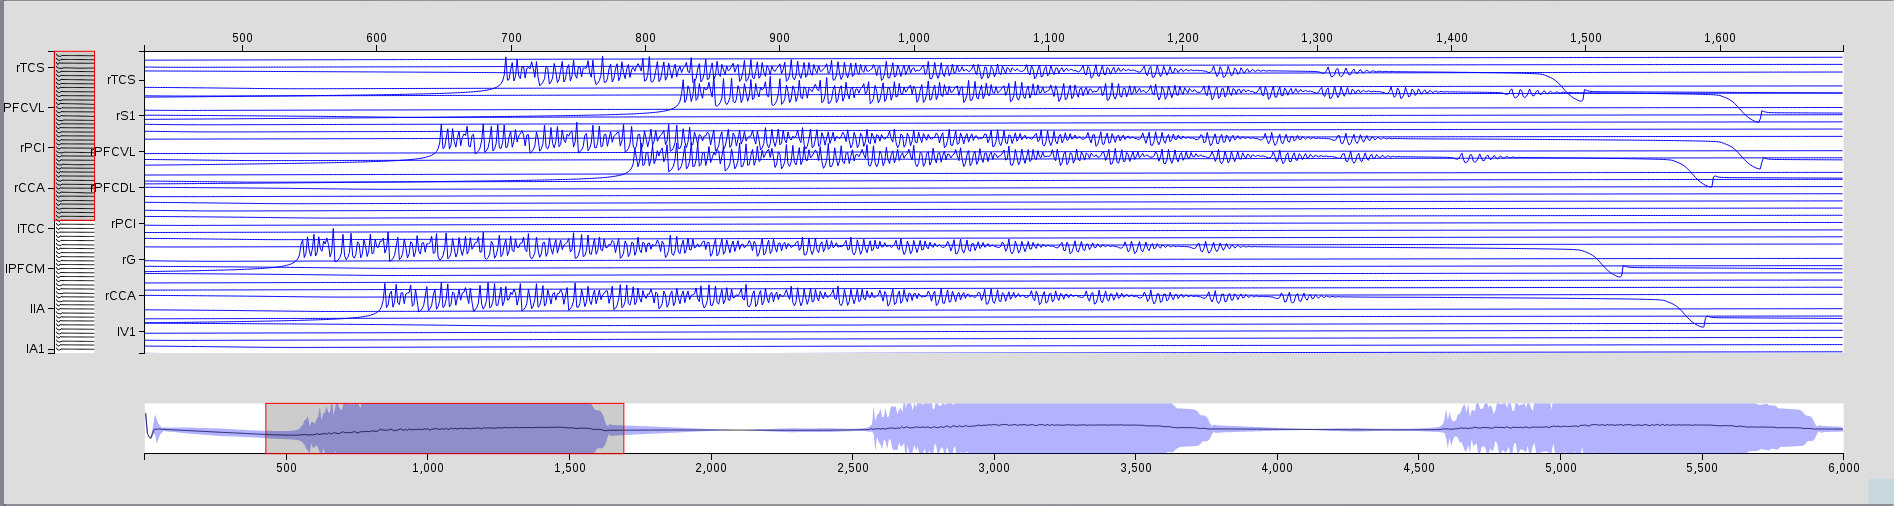
\includegraphics[width=\linewidth]{Handout_UI_ModellingAnEpilepticPatient_FirstPopulationTimesSeries}%
  \caption{Times series for the first population}%
  \label{fig:first_pop}%
\end{figure}

\begin{figure}[h]
  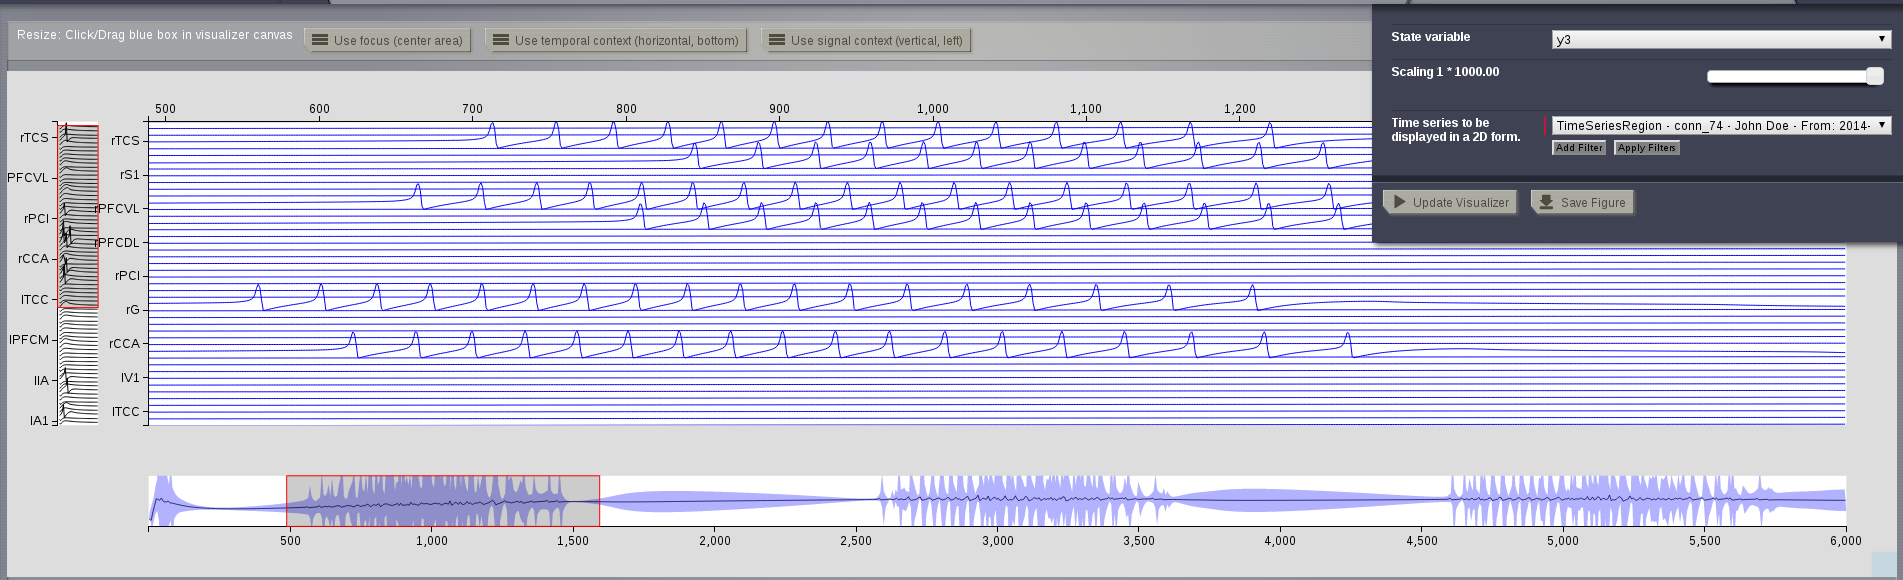
\includegraphics[width=\linewidth]{Handout_UI_ModellingAnEpilepticPatient_SecondPopulationTimesSeries}%
  \caption{Times series for the second population}%
  \label{fig:second_pop}%
\end{figure}

We now are going to rerun this simultion ,but with intracranial electrodes, EEG and MEG sensors.

\begin{simulation}
  \begin{enumerate}
  \item Copy the simulation
  \item add three new monitors (EEG, Spherical MEG and sEEG) by hittinh Ctrl and in the same time clicking on the monitors
  \item delete the brainviewer monitor otherwise you will have an error
  \item click on results
  \item visualize the sEEG with the 3d/2d vizualiser (Fig. \ref{fig:sEEG})
    \item visualize the sEEG with the 3d/2d vizualiser (Fig. \ref{fig:EEG})
\end{enumerate}
\end{simulation}

\begin{figure}[h]
  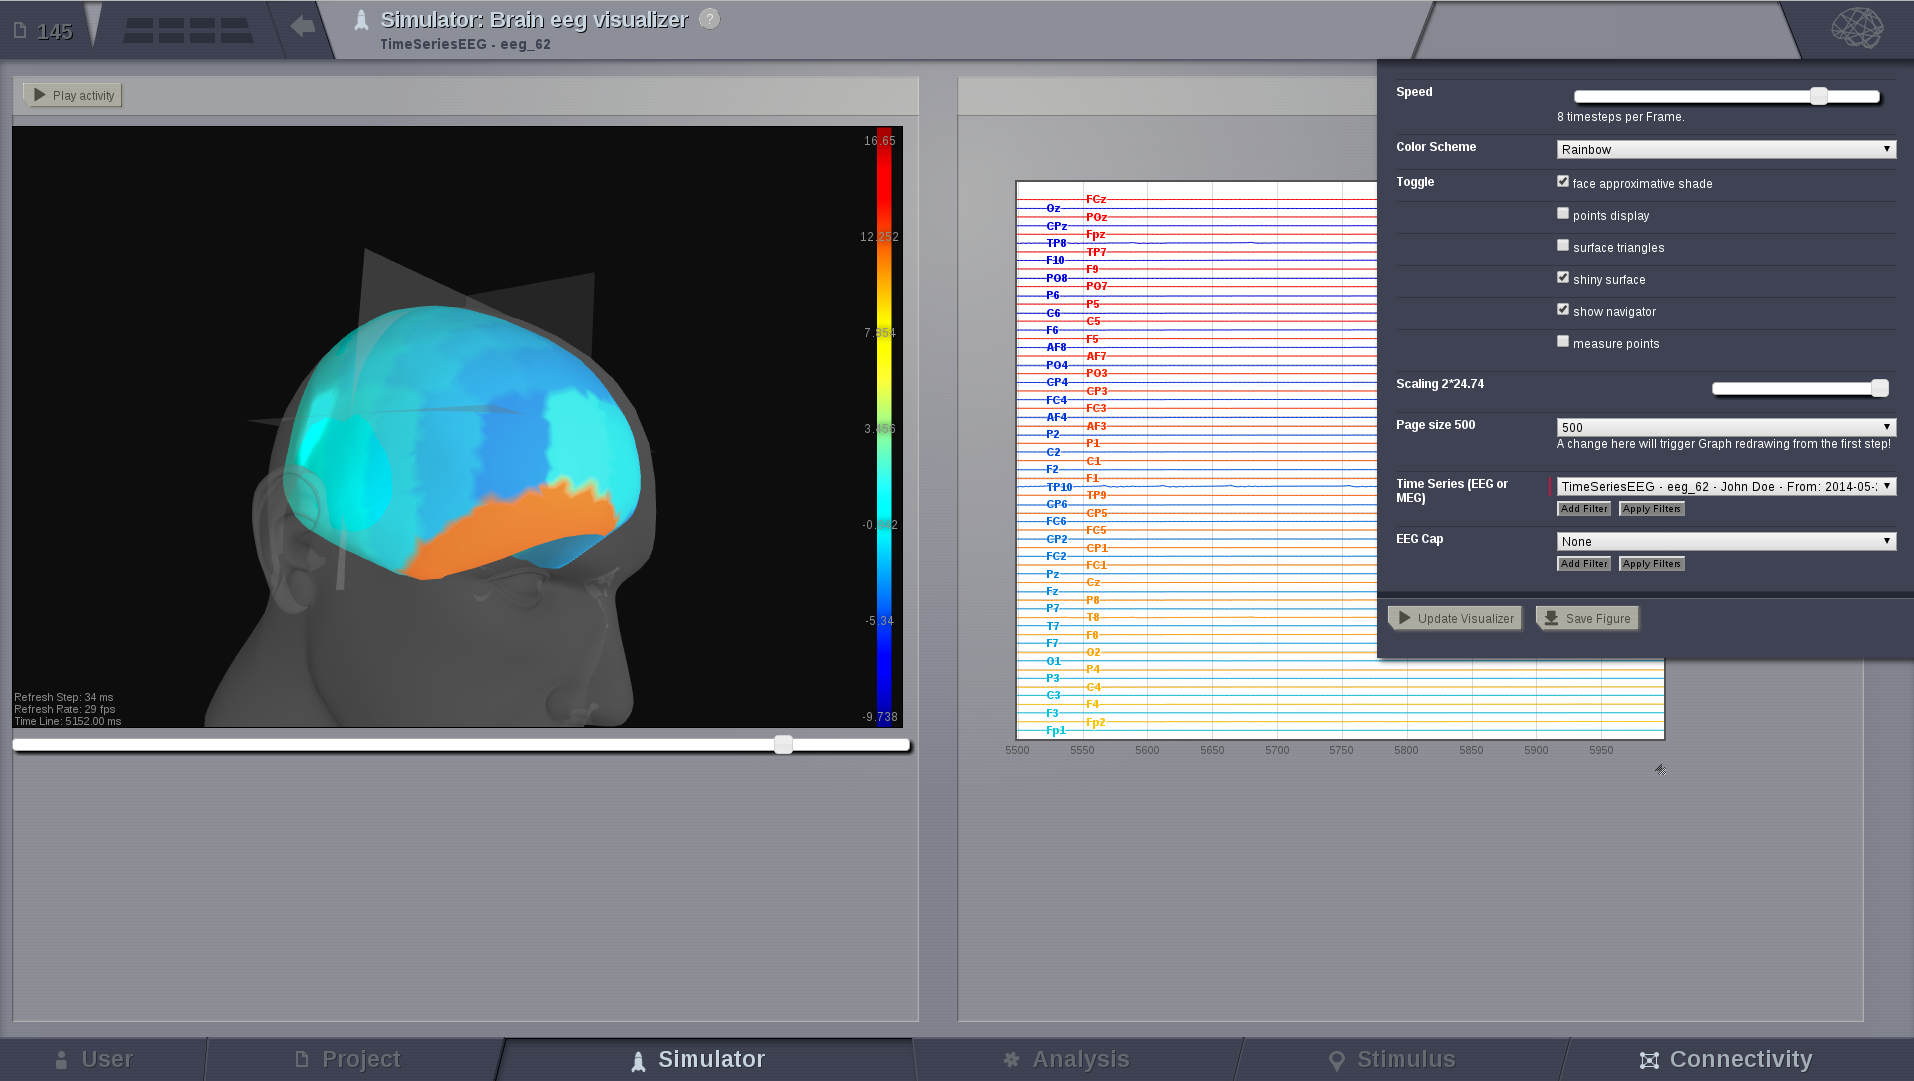
\includegraphics[width=\linewidth]{Handout_UI_ModellingAnEpilepticPatient_EEG3d2dBrainVizualiser}%
  \caption{sEEG 3d/2d vizualiser}%
  \label{fig:sEEG}%
\end{figure}

\begin{figure}[h]
  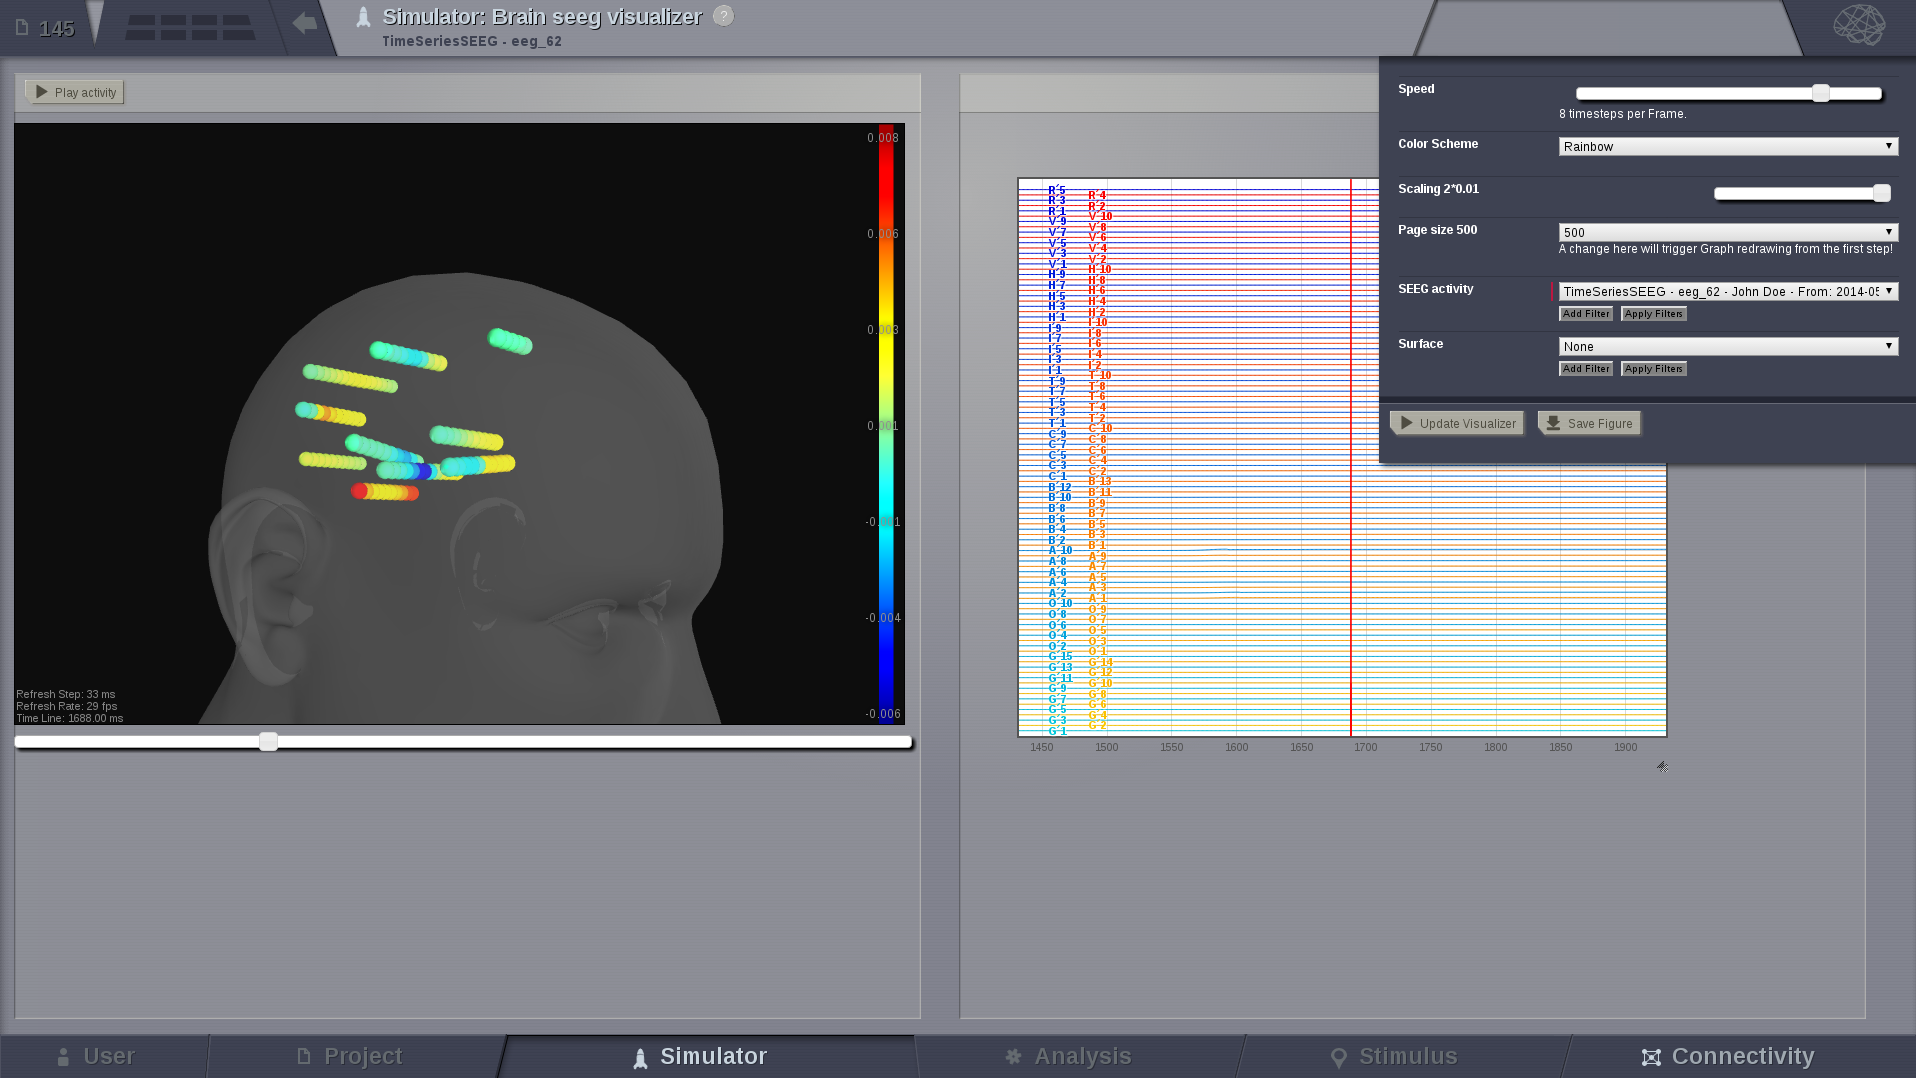
\includegraphics[width=\linewidth]{Handout_UI_ModellingAnEpilepticPatient_sEEG3d2dBrainVizualiser}%
  \caption{EEG 3d/2d vizualiser}%
  \label{fig:EEG}%
\end{figure}

\subsection{Steps: Surface Simulation}

 To account also for seizure propagtion and not only seizure recruitement, we have to use a seurace model. 
 It also help to have a more accurate representation of the EEG/sEEG signal
  \begin{simulation}
  \begin{enumerate}
  \item Copy the last simulation
  \item add a brainviewer monitor
  \item chose the surf reg 13
  \item choose the corresponding local connectivity
  \item choose  a coupling strength of 0.2
  \item add a temporal average vizualiser
  \item click on set up surface model (Fig. \ref{fig:set_up_surface_parameters})choose the good parameters (x0, amp 0.6, sigma 10.0, offset -2.2)and click on apply eqution. C	Click on a location on the brain where you wanthe parameter setting to apply, the click Add focal point.Then click on submit Surface parameters. You can see that the field x0 is updated with the relevant equation.
  \item visualize the sEEG with the 3d/2d vizualiser (Fig. \ref{fig:sEEG})
\end{enumerate}
\end{simulation}

\begin{figure}[h]
  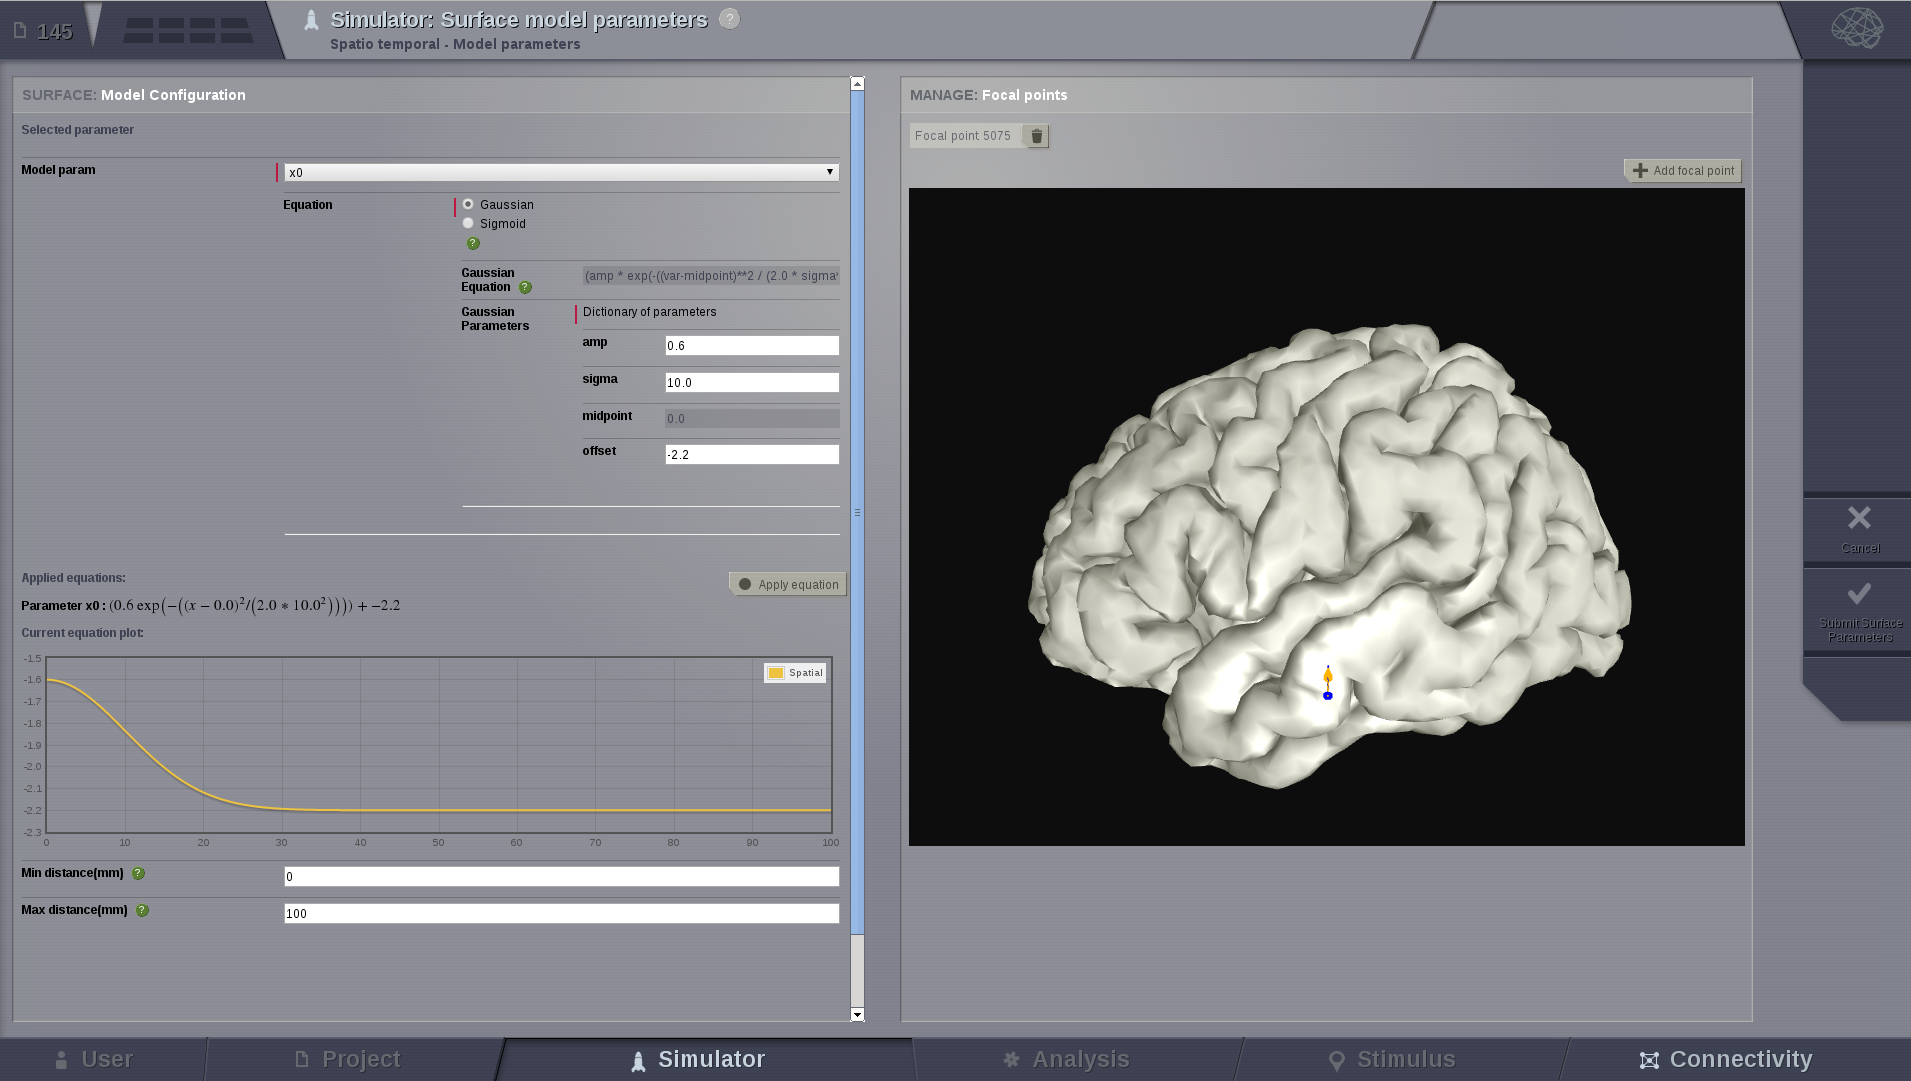
\includegraphics[width=\linewidth]{Handout_UI_ModellingAnEpilepticPatient_SetUpSurfaceParameters}%
  \caption{Set up the surface parameters}%
  \label{fig:set_up_surface_parameters}%
\end{figure}

\subsection{Steps: Simulating stimulation}

Now we are going to simulate a stimulation.
We use a stimulus prededined
We  set the whole brain to non-epileptogenic but close to the threshold

  \begin{simulation}
  \begin{enumerate}
  \item go to stimulus-Surface Stimulus
  \item give a name to the new stimulus
  \item choose a gaussian stimulation in space and in time (Fig. \ref{fig;stim_st})
  \item Click on view stimulus progress
  \item choose a focal point (Fig. \ref{fig;stim_foc})
  \item save the stimulus
  \item go to simulator, choose the stimulus you just defined
  \item set the parameter x0 to -2.1
 
\end{enumerate}
\end{simulation}

\begin{figure}[h]
  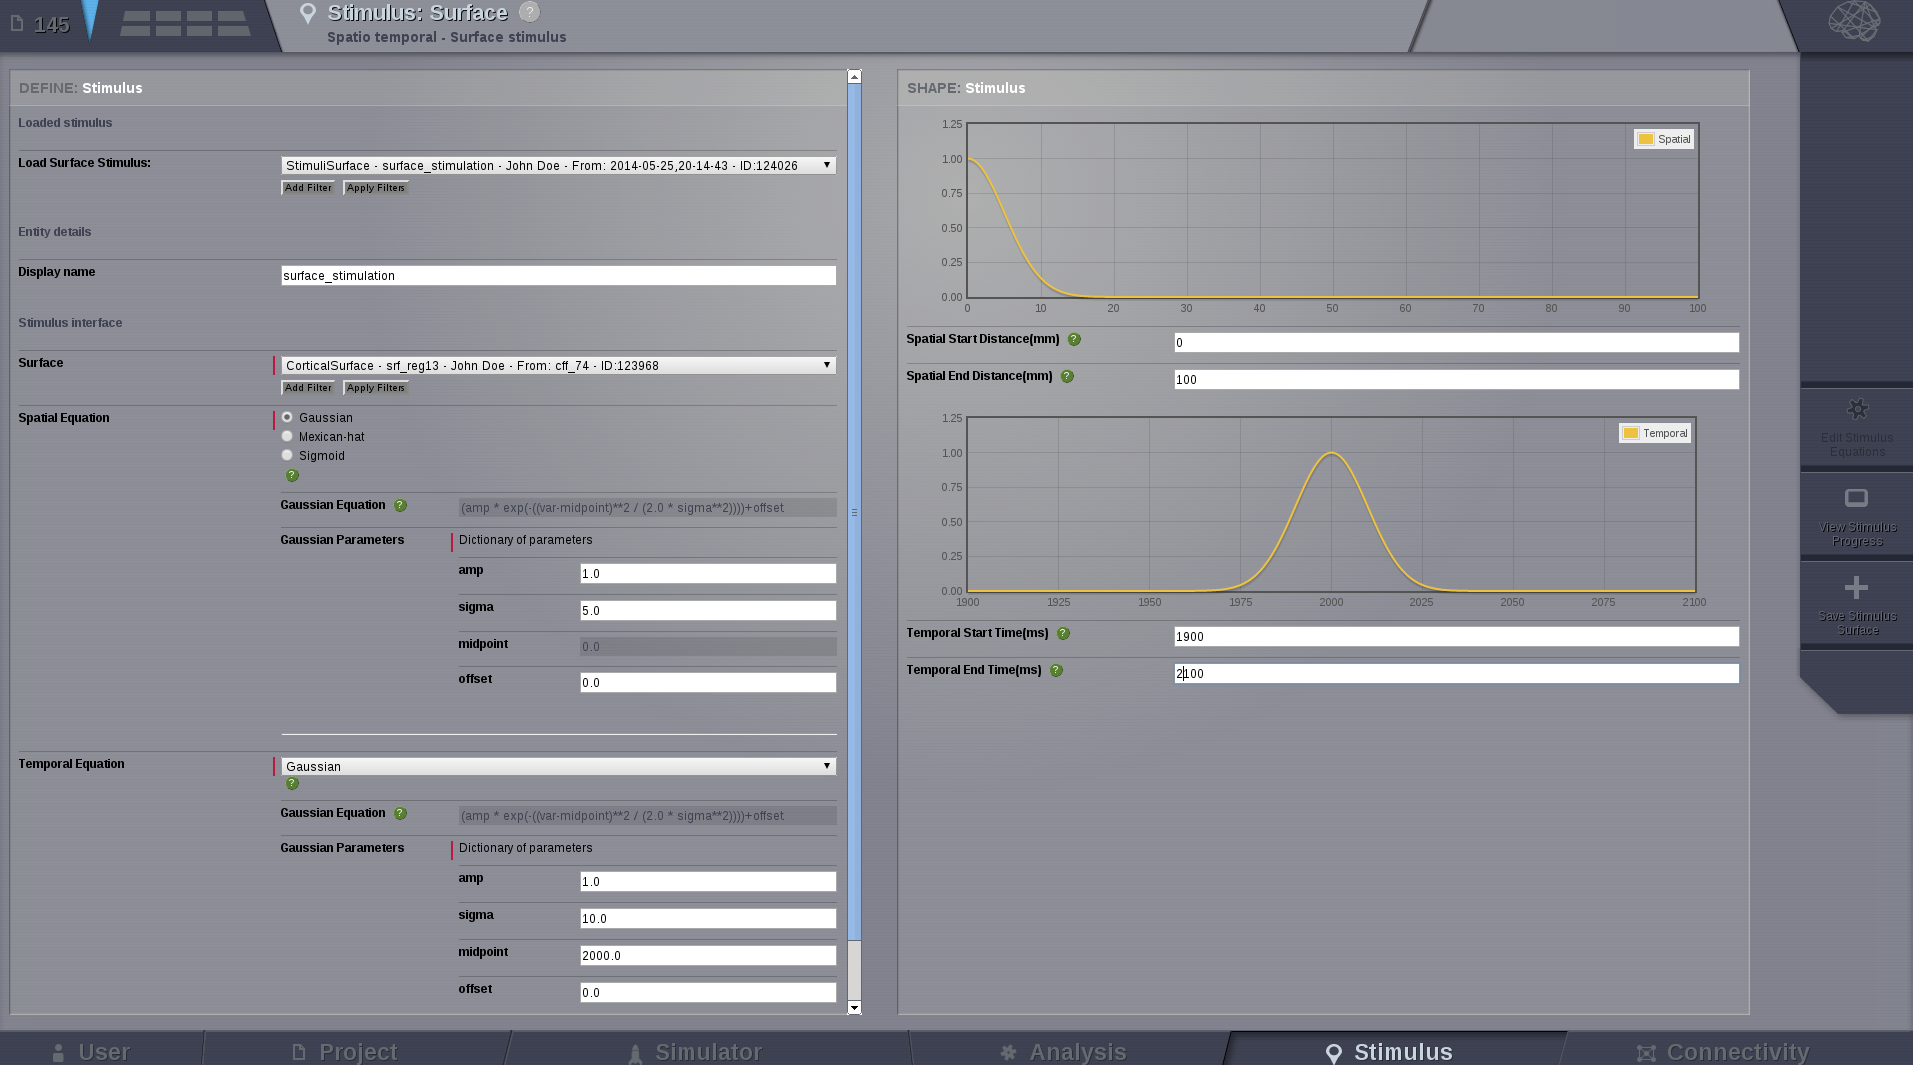
\includegraphics[width=\linewidth]{Handout_UI_ModellingAnEpilepticPatient_StimulationSpatioTemporalPattern}%
  \caption{Spatio temporal pattern of the stimulus}%
  \label{fig:stim_st}%
\end{figure}

\begin{figure}[h]
  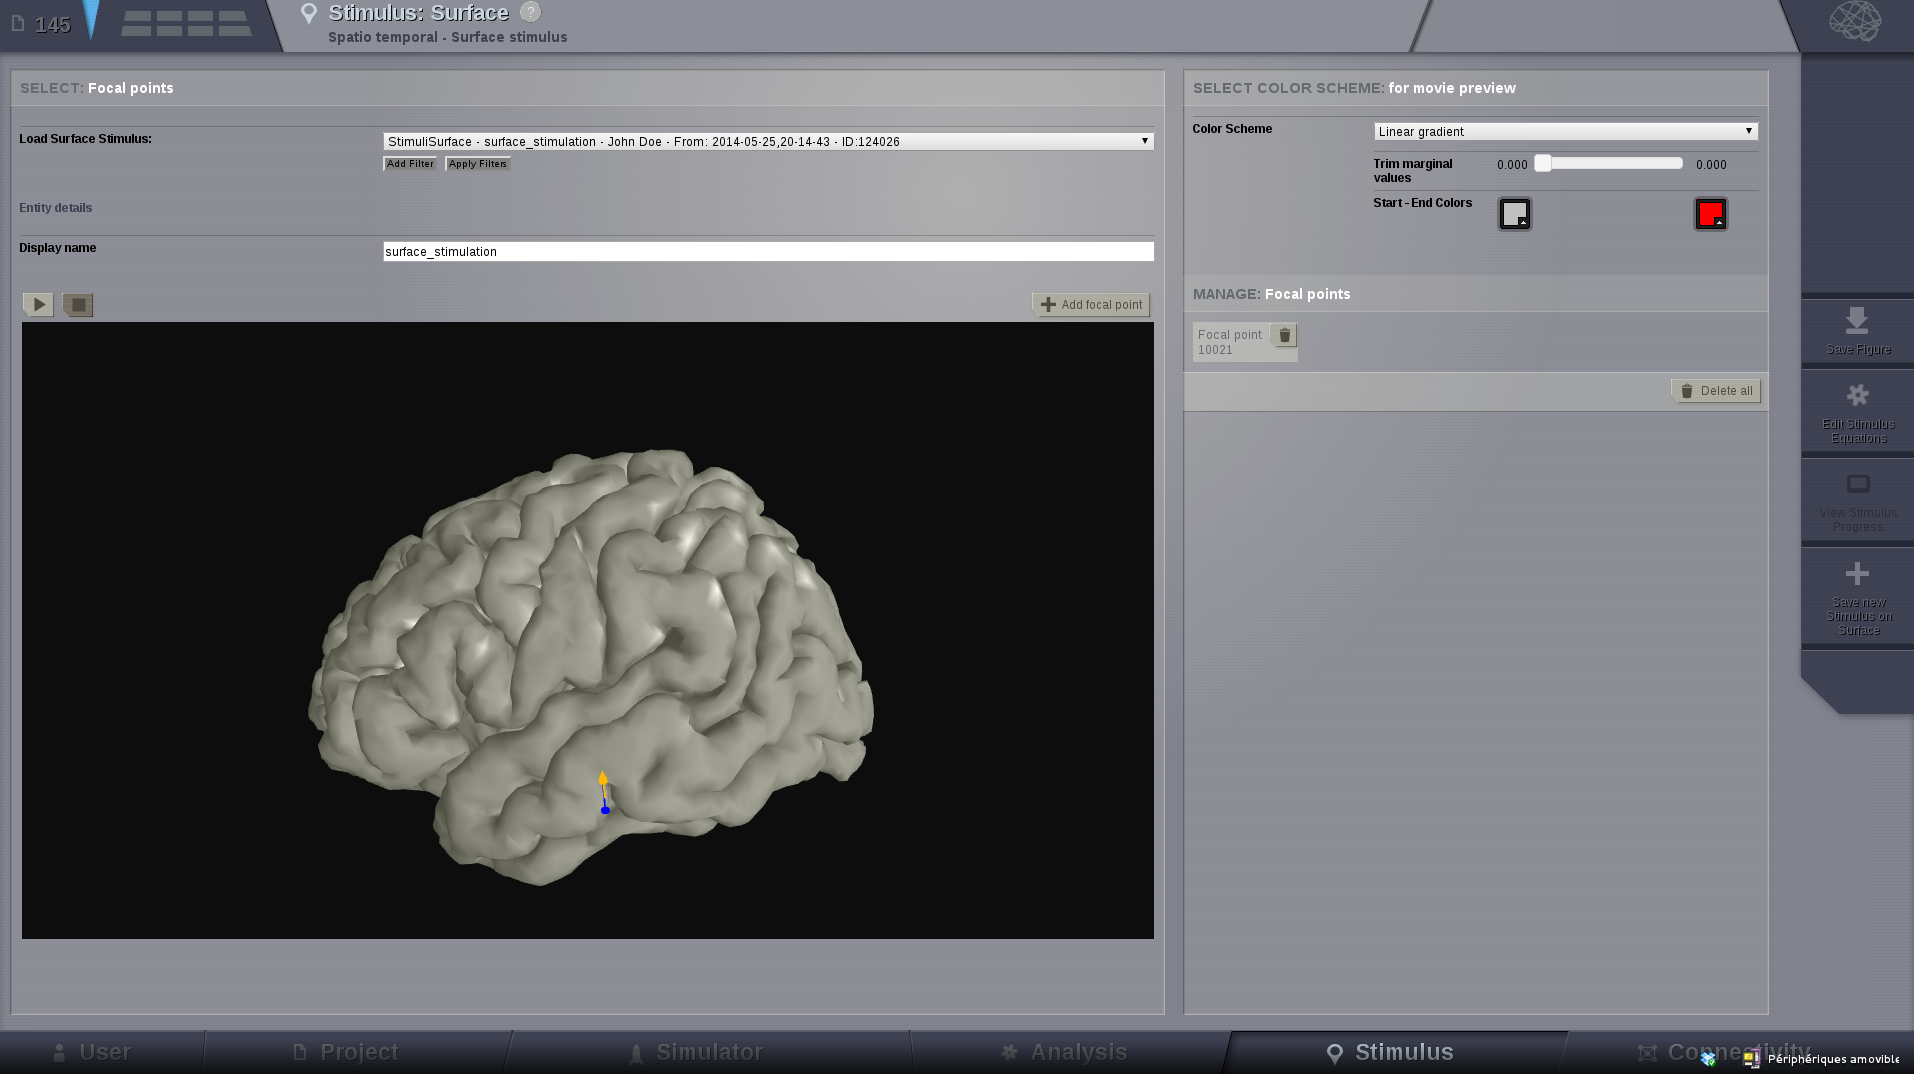
\includegraphics[width=\linewidth]{Handout_UI_ModellingAnEpilepticPatient_StimulationFocalPoint}%
  \caption{Focal point for a surface stimulation}%
  \label{fig:stim_foc}%
\end{figure}

You can view the result of this simulation in \textit{surface stimulation temporal\_lobe\_EEG\_sEEG\_MEG}
\subsection{Steps: Simulating Surface MEG spikes}

Often we do not have access with MEG to an epileptic seizure, but only to interictal periods.
Therefore it is interesting to simulate interictal spikes in order to test forward and inverse model in MEG.
WE are going to set hte parameter x0 in such a way that the epileptor will not have seizures, but only interictal spikes, 
i.e. close to the threshold. To have interictal spikes we need to add some noise.

  \begin{simulation}
  \begin{enumerate}
  \item As before, we are going to introduce an heterogeneity in the surface parameter, but without putting the node epileptogenic
  The setting is already done for you in the name simulation.
  \item We set a MEG monitors
  \item We look at the times series
\end{enumerate}
\end{simulation}

\subsection{Steps: Simulating resection}

Now we can simulate the effect of surgery. We can imagine in this case that a small part of the brain of the patients 
has been resected ( for instance the hippocampus, the amygdala and the parahippocampal cortex) and 
we are going to simulate that.

\begin{simulation}
  \begin{enumerate}
  \item go to connectivity-Large scale Connectivity
  \item As you learned in session III, select the nodes lAMYG, lHC and lPHC via your former selection,delete all their in-out and out-in connections
  with the other nodes, give a name to the selection and save it. (Fig. \ref{fig:resec})
  \item As we choose the same regional parameters that in the first simulation, we are going to copy them directly from our
  former setting. Go to the \textit{temporal lobe region} simulation, select and copy the vaues for the parameter  x0 
  \item copy the surface simulation \textit{Surface temporal lobe EEG MEG sEEG} and paste the values in the parameter x0.
  \item do not forget to choose the right connectivity matrix and you are ready to launch the simulation.
  \end{enumerate}
\end{simulation}

The results are given in \textit{surface resection tempoal lobe EEG MEG sEEG}.

\begin{figure}[h]
  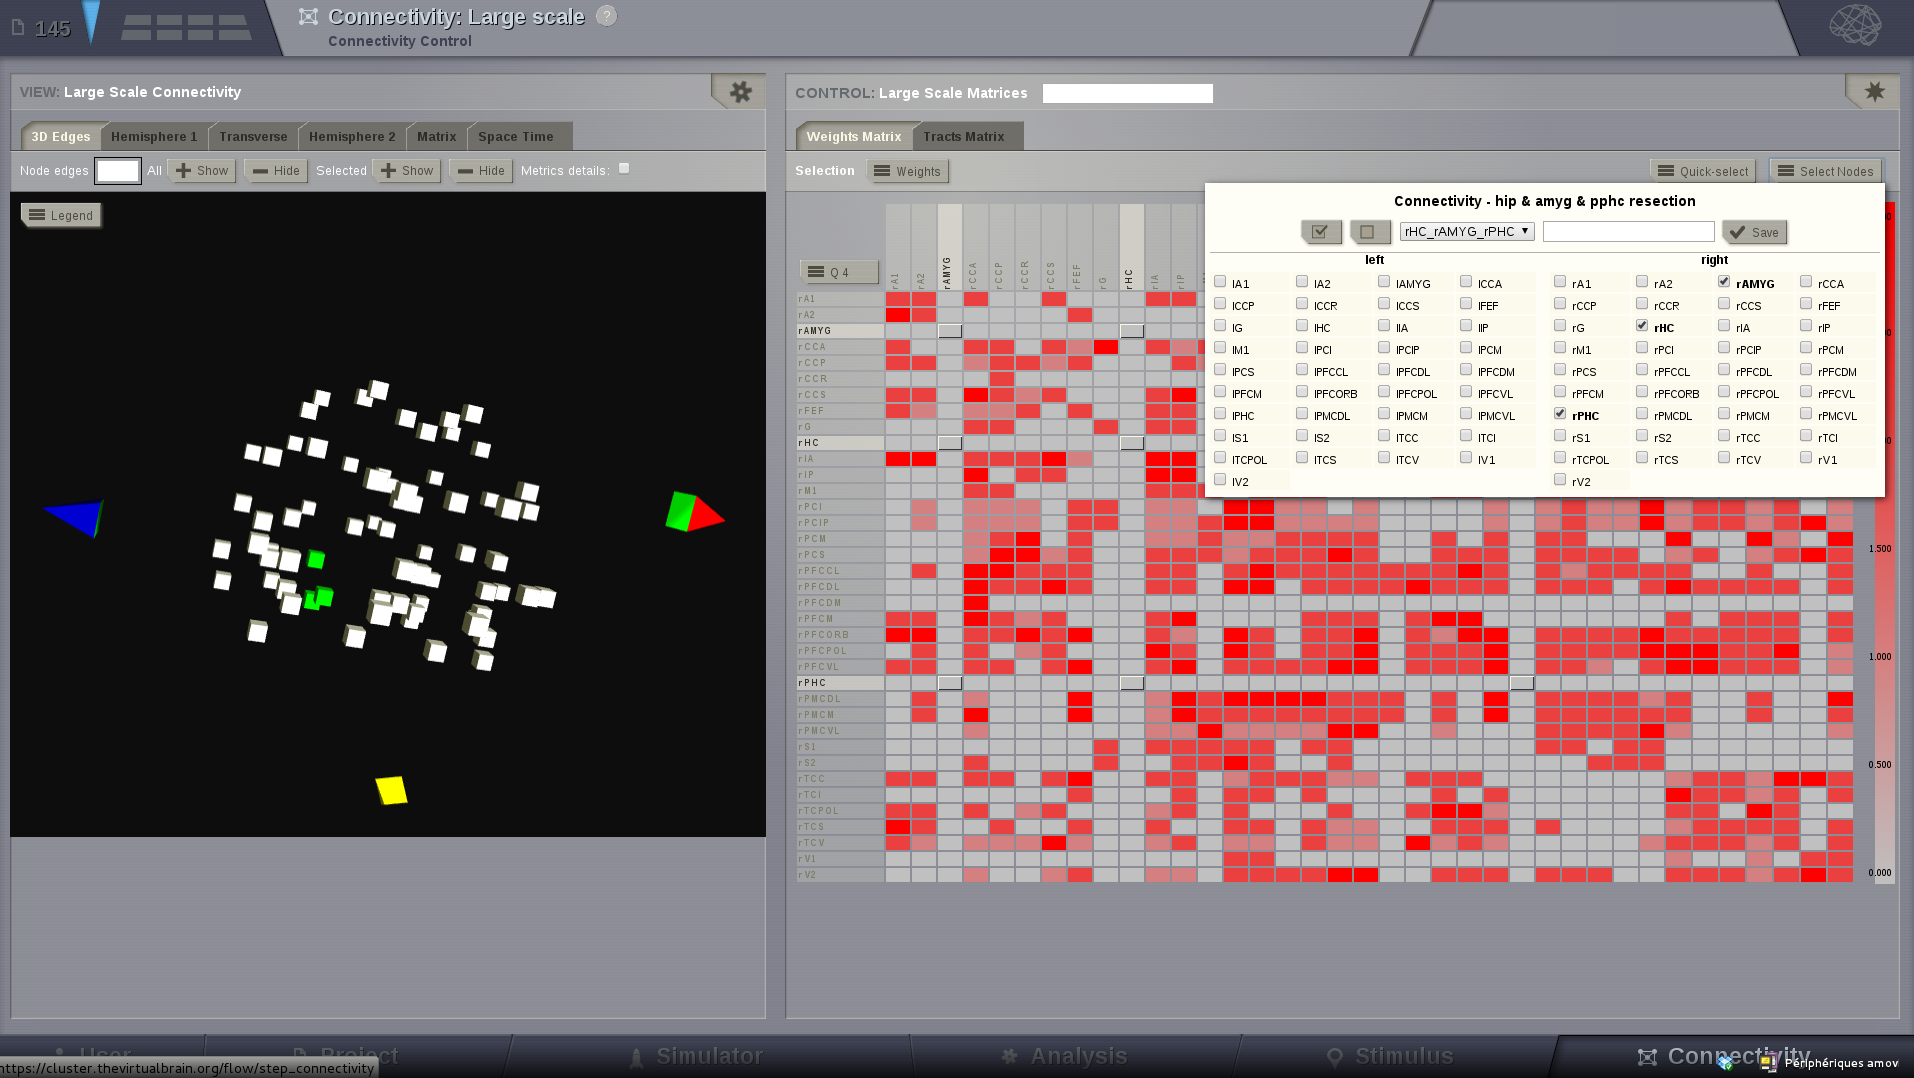
\includegraphics[width=\linewidth]{Handout_UI_ModellingAnEpilepticPatient_ConnectivityMatrixResection}%
  \caption{Focal point for a surface stimulation}%
  \label{fig:resec}%
\end{figure}

\section{More Documentation}\label{sec:more-doc}
For more documentation on The Virtual Brain, please see the following articles \cite{Sanz-Leon_2013, Spiegler_2013, Jirsa_2010b}


\section{Support}\label{sec:support}

The official TVB webiste is \url{www.thevirtualbrain.org}.  
All the documentation and tutorials are hosted on \url{the-virtual-brain.github.io}.
You'll find our public \smallcaps{git} repository at \url{https://github.com/the-virtual-brain}. For questions and bug reports we have a users group \url{https://groups.google.com/forum/#!forum/tvb-users}

\bibliography{tvb_references}
\bibliographystyle{plainnat}

\end{document}